% ============================================================
%  HJ-Biplot  —  TAM Questionnaire (n = 25)
%  System: AI-Powered Inclusive Mobile Messaging Application
%  Source: Figure 28, ProyectoFinal.pdf, p. 105
%    Dim 1: 43.6 %    Dim 2: 24.2 %    Cumulative: 67.8 %
%    UP  = Perceived Usefulness    (PTAM001-006)
%    FUP = Perceived Ease of Use   (PTAM007-012)
%
%  Visual encoding (matches fig3.pdf reference):
%    Dark-blue arrows  : UP items  (PTAM001-006) — main cluster
%    Red arrows        : FUP orthogonal items (PTAM007, 011, 012)
%    Gray arrows       : FUP non-orthogonal items (PTAM008-010)
%    Blue circles      : participants near UP cluster
%    Red circles       : participants in opposite quadrant (8,10,17,18,25)
%    Dashed ellipse    : UP cluster boundary
%    Red callout box   : orthogonal item label
%
%  All coordinates are LITERAL cm values (scale = 1.05 cm/unit).
%  Compilation: pdflatex  (requires tikz + arrows.meta)
% ============================================================

\documentclass[tikz, border=10pt]{standalone}

\usepackage{tikz}
\usetikzlibrary{arrows.meta, backgrounds}

% ── Colour palette ───────────────────────────────────────────
\definecolor{upblue}   {RGB}{ 30,  55, 110}   % UP arrows (dark navy)
\definecolor{orthored} {RGB}{190,  30,  45}   % orthogonal FUP arrows + red pts
\definecolor{fupgray}  {RGB}{145, 145, 145}   % non-orthogonal FUP arrows
\definecolor{ptblue}   {RGB}{ 65, 130, 200}   % participants near UP cluster
\definecolor{axisgray} {RGB}{150, 150, 150}   % axes and grid
\definecolor{gridgray} {RGB}{220, 220, 220}   % background grid
\definecolor{bgfill}   {RGB}{248, 248, 252}   % plot background
\definecolor{ellcol}   {RGB}{ 80,  80, 130}   % UP cluster ellipse

% ── Arrow / node styles ──────────────────────────────────────
\tikzset{
	up arrow/.style={
		-{Stealth[length=5.5pt, width=3.8pt]},
		line width=1.1pt, color=upblue,
	},
	orth arrow/.style={
		-{Stealth[length=6pt, width=4pt]},
		line width=1.5pt, color=orthored,
	},
	fup arrow/.style={
		-{Stealth[length=4.5pt, width=3pt]},
		line width=0.75pt, color=fupgray,
	},
	ax/.style={line width=0.5pt, color=axisgray},
	grid/.style={line width=0.4pt, color=gridgray},
	uppt/.style={circle, fill=ptblue,   inner sep=0pt, minimum size=5pt},
	rept/.style={circle, fill=orthored, inner sep=0pt, minimum size=5pt},
	ilab up/.style={font=\scriptsize\sffamily\bfseries, color=upblue,   inner sep=1pt},
	ilab or/.style={font=\scriptsize\sffamily\bfseries, color=orthored, inner sep=1pt},
	ilab fg/.style={font=\scriptsize\sffamily,          color=fupgray,  inner sep=1pt},
	plab/.style={font=\scriptsize\sffamily, color=black, inner sep=0.5pt},
}

% ── Shorthands ───────────────────────────────────────────────
\newcommand{\upvec}[4]  {\draw[up arrow]   (0,0)--(#2,#3); \node[ilab up, anchor=#4] at (#2,#3){#1};}
\newcommand{\orthvec}[4]{\draw[orth arrow] (0,0)--(#2,#3); \node[ilab or, anchor=#4] at (#2,#3){#1};}
\newcommand{\fupvec}[4] {\draw[fup arrow]  (0,0)--(#2,#3); \node[ilab fg, anchor=#4] at (#2,#3){#1};}

% Participant points: #1=number  #2=xcm  #3=ycm  #4=anchor
\newcommand{\bpp}[4]{\node[uppt] at (#2,#3){}; \node[plab, anchor=#4] at (#2,#3){\scriptsize #1};}
\newcommand{\rpp}[4]{\node[rept] at (#2,#3){}; \node[plab, anchor=#4] at (#2,#3){\scriptsize #1};}

\begin{document}
	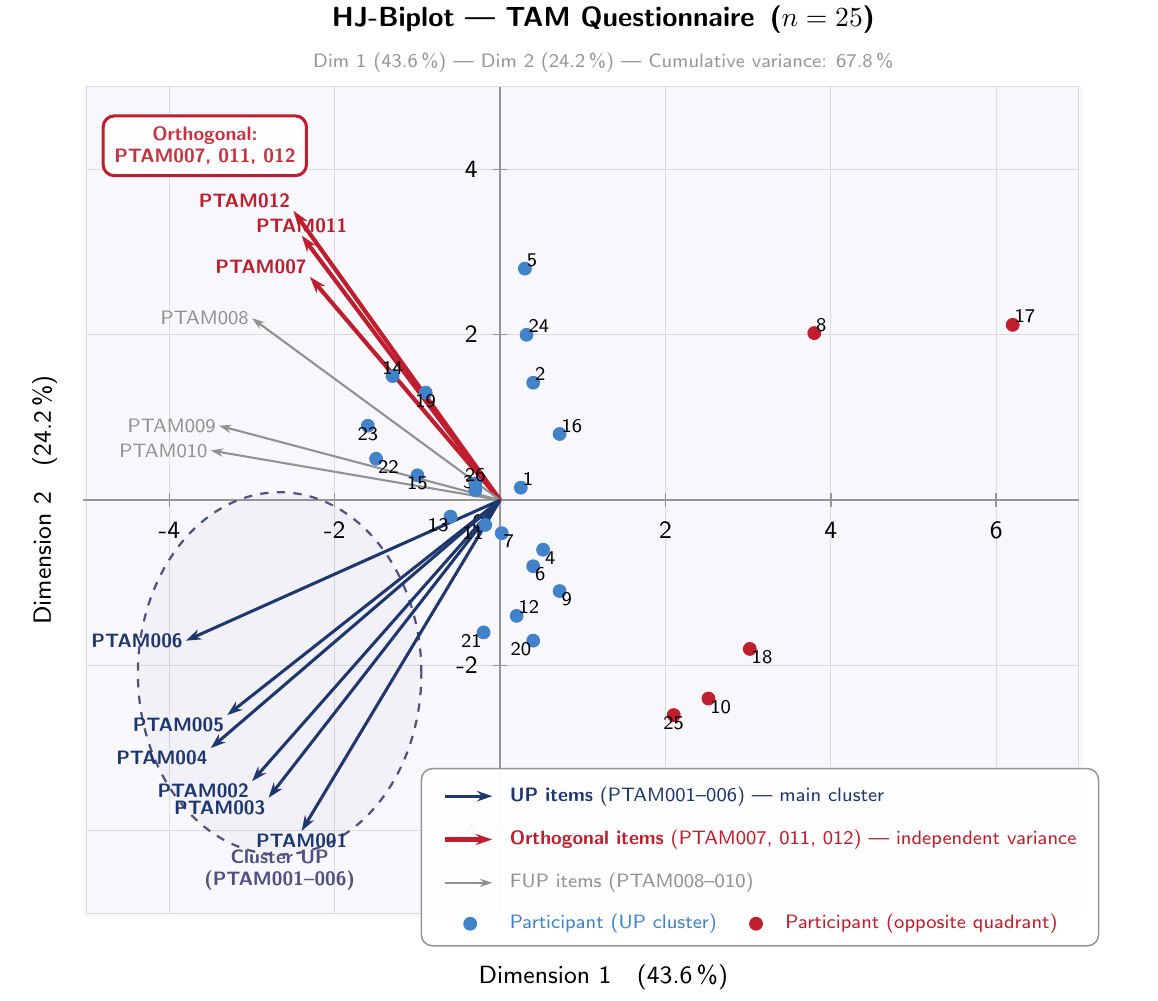
\begin{tikzpicture}
		
		% ============================================================
		% 1.  BOUNDING BOX
		% ============================================================
		\useasboundingbox (-6.0cm,-6.0cm) rectangle (8.0cm,6.0cm);
		
		% ============================================================
		% 2.  PLOT BACKGROUND + GRID
		% ============================================================
		\begin{scope}[on background layer]
			\fill[bgfill] (-5.3cm,-5.3cm) rectangle (7.4cm,5.25cm);
			% vertical grid lines
			\foreach \xc in {-5.25,-4.20,-2.10,0,2.10,4.20,6.30,7.35}{
				\draw[grid] (\xc,-5.25cm)--(\xc,5.26cm);
			}
			% horizontal grid lines
			\foreach \yc in {-5.25,-4.20,-2.10,0,2.10,4.20,5.25}{
				\draw[grid] (-5.25cm,\yc)--(7.35cm,\yc);
			}
		\end{scope}
		
		% ============================================================
		% 3.  AXES
		% ============================================================
		\draw[ax] (-5.3cm,0)--(7.35cm,0);
		\draw[ax] (0,-5.25cm)--(0,5.25cm);
		
		% x ticks
		\foreach \xc/\lbl in {-4.20/-4,-2.10/-2,2.10/2,4.20/4,6.30/6}{
			\draw[ax] (\xc,-0.09cm)--(\xc,0.09cm);
			\node[font=\small\sffamily, below=2pt] at (\xc,-0.09cm) {\lbl};
		}
		\node[font=\small\sffamily, below left=2pt] at (0,0) {0};
		
		% y ticks
		\foreach \yc/\lbl in {-4.20/-4,-2.10/-2,2.10/2,4.20/4}{
			\draw[ax] (-0.09cm,\yc)--(0.09cm,\yc);
			\node[font=\small\sffamily, left=2pt] at (-0.09cm,\yc) {\lbl};
		}
		
		% Axis labels
		\node[font=\small\sffamily, below=22pt] at (1.31cm,-5.cm)
		{Dimension~1\quad(43.6\,\%)};
		\node[font=\small\sffamily, rotate=90, above=22pt] at (-4.73cm,0)
		{Dimension~2\quad(24.2\,\%)};
		
		% ============================================================
		% 4.  UP CLUSTER ELLIPSE  (dashed, around PTAM001-006 vectors)
		% ============================================================
		\draw[dashed, line width=0.8pt, color=ellcol, fill=ellcol, fill opacity=0.04]
		(-2.80cm,-2.20cm) ellipse (1.80cm and 2.30cm);
		\node[font=\scriptsize\sffamily\bfseries, color=ellcol, align=center]
		at (-2.80cm,-4.70cm) {Cluster UP\\(PTAM001--006)};
		
		% ============================================================
		% 5.  ITEM VECTORS
		% ============================================================
		
		% ── Orthogonal FUP items: PTAM007, PTAM011, PTAM012  (RED) ──
		\orthvec{PTAM012}{-2.625cm}{ 3.675cm}{south east}
		\orthvec{PTAM011}{-2.520cm}{ 3.360cm}{south}
		\orthvec{PTAM007}{-2.415cm}{ 2.835cm}{south east}
		
		% ── Non-orthogonal FUP items: PTAM008, 009, 010  (GRAY) ──────
		\fupvec{PTAM008}{-3.150cm}{ 2.310cm}{east}
		\fupvec{PTAM009}{-3.570cm}{ 0.945cm}{east}
		\fupvec{PTAM010}{-3.675cm}{ 0.630cm}{east}
		
		% ── UP items: PTAM001-006  (DARK BLUE) ───────────────────────
		\upvec{PTAM006}{-3.990cm}{-1.785cm}{east}
		\upvec{PTAM005}{-3.465cm}{-2.730cm}{north east}
		\upvec{PTAM002}{-3.150cm}{-3.570cm}{north east}
		\upvec{PTAM001}{-2.520cm}{-4.200cm}{north}
		\upvec{PTAM003}{-2.940cm}{-3.780cm}{north east}
		\upvec{PTAM004}{-3.675cm}{-3.150cm}{north east}
		
		% ============================================================
		% 6.  ORTHOGONAL CALLOUT BOX  (red rounded rectangle)
		% ============================================================
		\node[draw=orthored, fill=white, fill opacity=0.90,
		rounded corners=4pt, line width=1.1pt,
		font=\scriptsize\sffamily\bfseries, text=orthored,
		align=center, inner sep=4pt]
		at (-3.75cm, 4.5cm)
		{Orthogonal:\\PTAM007, 011, 012};
		
		% ============================================================
		% 7.  PARTICIPANT POINTS
		%     Blue  = near UP cluster (most participants)
		%     Red   = opposite quadrant (8, 10, 17, 18, 25)
		% ============================================================
		
		% ── Blue participants ─────────────────────────────────────────
		\bpp{1} { 0.263cm}{ 0.158cm}{south west}
		\bpp{2} { 0.420cm}{ 1.491cm}{south west}
		\bpp{3} {-0.315cm}{ 0.126cm}{south east}
		\bpp{4} { 0.546cm}{-0.630cm}{north west}
		\bpp{5} { 0.315cm}{ 2.940cm}{south west}
		\bpp{6} { 0.420cm}{-0.840cm}{north west}
		\bpp{7} { 0.021cm}{-0.420cm}{north west}
		\bpp{9} { 0.756cm}{-1.155cm}{north west}
		\bpp{11}{-0.189cm}{-0.315cm}{north east}
		\bpp{12}{ 0.210cm}{-1.470cm}{south west}
		\bpp{13}{-0.630cm}{-0.210cm}{north east}
		\bpp{14}{-1.365cm}{ 1.575cm}{south}
		\bpp{15}{-1.050cm}{ 0.315cm}{north}
		\bpp{16}{ 0.756cm}{ 0.840cm}{south west}
		\bpp{19}{-0.945cm}{ 1.365cm}{north}
		\bpp{20}{ 0.420cm}{-1.785cm}{north east}
		\bpp{21}{-0.210cm}{-1.680cm}{north east}
		\bpp{22}{-1.575cm}{ 0.525cm}{north west}
		\bpp{23}{-1.680cm}{ 0.945cm}{north}
		\bpp{24}{ 0.336cm}{ 2.100cm}{south west}
		\bpp{26}{-0.315cm}{ 0.210cm}{south}
		
		% ── Red participants (opposite quadrant) ─────────────────────
		\rpp{8} { 3.990cm}{ 2.121cm}{south west}
		\rpp{10}{ 2.646cm}{-2.520cm}{north west}
		\rpp{17}{ 6.510cm}{ 2.226cm}{south west}
		\rpp{18}{ 3.171cm}{-1.890cm}{north west}
		\rpp{25}{ 2.205cm}{-2.730cm}{north}
		
		% ============================================================
		% 8.  LEGEND  (4 entries, positioned bottom-right)
		%     shift = literal cm, no arithmetic
		% ============================================================
		\begin{scope}[shift={(-0.50cm,-5.460cm)}]
			\draw[line width=0.55pt, color=axisgray,
			fill=white, fill opacity=0.97, rounded corners=4pt]
			(-0.5cm,-0.20cm) rectangle (8.10cm,2.05cm);
			
			% Row 1: UP arrows
			\draw[up arrow, line width=1.1pt] (-0.2cm,1.70cm)--(0.4cm,1.70cm);
			\node[font=\scriptsize\sffamily, anchor=west, color=upblue] at (0.50cm,1.70cm)
			{\textbf{UP items} (PTAM001--006) --- main cluster};
			
			% Row 2: orthogonal red arrows
			\draw[orth arrow] (-0.2cm,1.15cm)--(0.4cm,1.15cm);
			\node[font=\scriptsize\sffamily, anchor=west, color=orthored] at (0.50cm,1.15cm)
			{\textbf{Orthogonal items} (PTAM007, 011, 012) --- independent variance};
			
			% Row 3: gray FUP arrows
			\draw[fup arrow] (-0.2cm,0.60cm)--(0.4cm,0.60cm);
			\node[font=\scriptsize\sffamily, anchor=west, color=fupgray] at (0.50cm,0.60cm)
			{FUP items (PTAM008--010)};
			
			% Row 4a: blue participant
			\node[uppt] at (0.12cm,0.08cm){};
			\node[font=\scriptsize\sffamily, anchor=west, color=ptblue] at (0.5cm,0.08cm)
			{Participant (UP cluster)};
			
			% Row 4b: red participant (same row, right side)
			\node[rept] at (3.75cm,0.08cm){};
			\node[font=\scriptsize\sffamily, anchor=west, color=orthored] at (4.0cm,0.08cm)
			{Participant (opposite quadrant)};
		\end{scope}
		
		% ============================================================
		% 9.  TITLE  (two lines matching the reference)
		% ============================================================
		\node[font=\normalsize\bfseries\sffamily, anchor=south] at (1.31cm,5.80cm)
		{HJ-Biplot --- TAM Questionnaire\enspace($n = 25$)};
		\node[font=\scriptsize\sffamily, color=axisgray, anchor=north] at (1.31cm,5.80cm)
		{Dim 1 (43.6\,\%) --- Dim 2 (24.2\,\%) --- Cumulative variance: 67.8\,\%};
		
	\end{tikzpicture}
\end{document}